% =============================================================================
%  Retrieval or Ranking? Diagnosing the Dominant Bottleneck in a Hybrid
%  Two-Stage Recommender on a Sparse Product Catalogue
%  Emmanuel Boakye, Loughborough University
%
%  Every numeric value was verified against pipeline artefacts by
%  verify_paper_numbers.py, final_results_table.py, make_new_figures.py and
%  ml_density_check.py. Figures: 6. Tables: 8.
% =============================================================================

\documentclass[10pt,twocolumn]{article}

\usepackage[utf8]{inputenc}
\usepackage[T1]{fontenc}
\usepackage[british]{babel}
% mathptmx, not times. The times package sets Times for text only and leaves
% maths in Computer Modern, so formulas render in a different typeface from
% the body. mathptmx sets both, which keeps the two consistent.
\usepackage{mathptmx}
\usepackage[margin=0.75in]{geometry}
\usepackage{amsmath,amssymb}
\usepackage{graphicx}
\usepackage{booktabs}
\usepackage{tabularx}
\usepackage{titlesec}
\usepackage{fancyhdr}
% APA reference list and APA author-year citations. apacite is loaded with
% natbibapa so the existing \citet and \citep commands keep working: \citet
% gives "Covington et al. (2016)" and \citep gives "(Covington et al., 2016)".
% Do not also load natbib; apacite supplies those commands itself.
\usepackage[natbibapa]{apacite}
\usepackage{caption}
\usepackage{microtype}
\usepackage[hidelinks]{hyperref}

\bibliographystyle{apacite}

% Figures live in figures/ alongside this file. Keep the trailing slash and
% the double braces, or Overleaf will not find them.
\graphicspath{{figures/}}

% ---- vertical spacing -------------------------------------------------------
% All spacing is set once here. Do not add \vspace inside the body: ad-hoc
% nudges are what makes spacing look uneven from one page to the next.
%
% \raggedbottom is the important one. In twocolumn LaTeX defaults to
% \flushbottom, which forces both columns to end at the same depth by
% stretching whatever vertical glue it can find, including the space between
% paragraphs. That is what produces small, varying gaps before paragraphs.
% \raggedbottom lets a column end short instead, so paragraph spacing stays
% exactly as specified. The glue below is given zero stretch for the same
% reason.
\raggedbottom
% Block paragraphs: no first-line indent, a small gap instead. The stretch is
% deliberately tiny, because \raggedbottom above is what stops TeX abusing it
% to pad columns out to equal depth.
\setlength{\parindent}{0pt}
\setlength{\parskip}{0.55em plus 0.1em minus 0.05em}

\captionsetup{font=small,labelfont=bf,skip=4pt}
\setlength{\abovedisplayskip}{5pt plus 1pt minus 1pt}
\setlength{\belowdisplayskip}{5pt plus 1pt minus 1pt}
\setlength{\abovedisplayshortskip}{3pt plus 1pt minus 1pt}
\setlength{\belowdisplayshortskip}{3pt plus 1pt minus 1pt}
\setlength{\textfloatsep}{10pt plus 2pt minus 2pt}
\setlength{\floatsep}{10pt plus 2pt minus 2pt}
\setlength{\intextsep}{10pt plus 2pt minus 2pt}

% ---- line breaking ----------------------------------------------------------
% A narrow twocolumn measure makes TeX hyphenate aggressively. Penalising
% hyphenation and allowing a little extra stretch on the worst lines removes
% most broken words; microtype then absorbs the slack by micro-adjusting
% character widths rather than by widening word spaces.
\hyphenpenalty=5000
\exhyphenpenalty=5000
\tolerance=3000
\setlength{\emergencystretch}{4em}
\clubpenalty=10000
\widowpenalty=10000

% ---- tables -----------------------------------------------------------------
% One set of metrics for every table so none needs shrinking to fit, and all
% render at the same size. Tables are set with tabularx below so that each one
% spans the full width of whatever it sits in, column or page, instead of
% floating narrow in the middle.
\setlength{\tabcolsep}{4pt}
\renewcommand{\arraystretch}{1.10}

% L is a left-aligned stretching column. It absorbs the slack so the numeric
% columns stay tight and the rule spans the full measure. R right-aligns.
\newcolumntype{L}{>{\raggedright\arraybackslash}X}
\newcolumntype{R}{>{\raggedleft\arraybackslash}X}

\titleformat{\section}{\normalfont\large\bfseries}{\thesection.}{0.5em}{\MakeUppercase}
\titleformat{\subsection}{\normalfont\normalsize\bfseries}{\thesubsection}{0.5em}{}
% The third value is the gap under the heading. It is small because \parskip
% above adds to it; raising either one makes headings float away from their
% text.
\titlespacing*{\section}{0pt}{9pt}{2pt}
\titlespacing*{\subsection}{0pt}{7pt}{1pt}
\titlespacing*{\subsubsection}{0pt}{6pt}{1pt}

\pagestyle{fancy}
\fancyhf{}
\fancyhead[L]{\small Retrieval or Ranking?}
\fancyhead[R]{\small E. Boakye}
\fancyfoot[C]{\small\thepage}
\renewcommand{\headrulewidth}{0pt}

\newcommand{\Lobs}{\mathcal{L}_{\mathrm{obs}}}
\newcommand{\Lalign}{\mathcal{L}_{\mathrm{align}}}

% Front matter after the abstract (CCS, keywords). One definition so the two
% blocks are separated identically instead of by hand-tuned \vspace.
\newenvironment{frontmatterblock}
  {\par\addvspace{0.6em}\small\setlength{\parskip}{0.4em}}
  {\par\addvspace{0.6em}}

\title{\vspace{-2em}\textbf{Retrieval or Ranking? Diagnosing the Dominant
Bottleneck in a Hybrid Two-Stage Recommender on a Sparse Product
Catalogue}\vspace{-0.5em}}
\author{Emmanuel Boakye\\
\small Department of Computer Science, Loughborough University, UK}
\date{}

\begin{document}
\maketitle
\thispagestyle{fancy}

% =============================================================================
\begin{abstract}
\small
Two-stage recommender systems separate candidate retrieval from ranking to
handle large catalogues, yet the coupling between the stages is rarely
measured directly. We build a hybrid two-stage system combining collaborative,
semantic and item-to-item signals, evaluate it on the Amazon Electronics
Reviews 2023 dataset under a leakage-controlled protocol, and measure each
stage independently. Training the ranker on observed rated pairs mismatches
the retrieved candidate distribution it must score at inference. Training on
retrieved candidates instead raises the top-ten hit rate from 17\% to 52\% in
isolation, with the same model and features. It also decides whether the
system beats a non-personalised popularity baseline. Scored on one candidate
pool, popularity outperforms the uncorrected ranker threefold and loses to the
corrected one by 0.0610 at HR@10. Feature attributions temper that result. The
corrected ranker draws 84.3\% of its split gain from item popularity against
31.3\% before correction, so alignment appears to teach a popularity prior and
a modest correction to it, at a measurable cost in concentration. Retrieval
rather than ranking is the dominant bottleneck here. Recall reaches only
3.30\% at 200 candidates and does not saturate. Injecting the held-out item
while holding the ranker fixed multiplies HR@10 by 8.3, with a near-linear
dose response. Even then, the ranker misses that item from its top ten in
84\% of cases. A supplementary evaluation finds cold-start covers 70\% of
users and 83\% of items, with the semantic signal reaching cold items but not
cold users.
\end{abstract}

\begin{frontmatterblock}
\noindent\textbf{CCS Concepts:}
$\bullet$ Information systems $\rightarrow$ Recommender systems;
Retrieval models and ranking;
$\bullet$ Computing methodologies $\rightarrow$ Learning to rank;
Supervised learning.

\noindent\textbf{Keywords:} two-stage recommendation, retrieval-ranking,
training-serving alignment, cold-start, LambdaRank, collaborative filtering
\end{frontmatterblock}

% =============================================================================
\section{Introduction}
\label{sec:intro}

Two-stage recommender systems, which separate candidate retrieval from final
ranking, have become the standard architecture for recommendation at scale
\citep{covington2016deep,huang2025survey}. The design reflects a practical
division of labour where a retrieval stage quickly searches a catalogue of
millions and a ranking stage orders a small candidate set precisely. Despite
wide adoption, three aspects of how these systems behave receive insufficient
empirical attention.

First, the two stages are typically designed and evaluated in isolation. This
hides a structural dependency. The ranking stage can only order items
retrieval has already returned, so retrieval recall imposes a hard ceiling on
end-to-end performance \citep{huang2025survey}. Whether retrieval recall is
the dominant bottleneck on sparse data, and what follows when it is, has not
been established through stage-separated measurement.

Second, ranking models in two-stage systems are commonly trained on observed
user-item interactions while at inference they score the candidates retrieval
supplies. These distributions differ. The effect of this mismatch on ranking
quality has been studied where retrieval is effective
\citep{kang2019candidate,zheng2024full}, but not in the regime where retrieval
recall is low and the candidate pool is impoverished.

Third, cold-start is treated as an edge case in most evaluations, yet the
$k$-core filtering standard in the literature removes cold users and items by
construction. The scale of the cold regime on realistically sparse data, and
whether cold items and cold users are equally tractable, is rarely quantified.

This paper addresses all three by building a hybrid two-stage recommender and
evaluating it under a leakage-controlled protocol that separates retrieval
from ranking. The contributions are:

\begin{enumerate}\itemsep2pt
\item Retrieval recall is shown to be the dominant bottleneck on this
catalogue. Injecting the held-out item into the candidate pool while holding
the ranker fixed raises HR@10 by a factor of 8.3, and the response is close to
linear in injection probability, so recall converts to ranking gain at a
near-constant rate with no saturation in the measured range.

\item Aligning the ranker's training distribution with its serving
distribution raises the top-ten hit rate from 17\% to 52\% in isolation with
the same model and features, and it is what decides whether the system
outperforms a non-personalised popularity baseline. Feature attributions
indicate that the corrected ranker is popularity-dominated, which qualifies
how the gain should be interpreted.

\item The cold-start regime accounts for 70\% of users and 83\% of items, and
a structural asymmetry is identified. The semantic signal extends to cold
items but not to cold users.
\end{enumerate}

Throughout, the protocol is leakage-controlled and stage-separated, and
uncertainty is reported over both model initialisation and the draw of
evaluation negatives.

% =============================================================================
\section{Related Work}
\label{sec:related}

This section reviews prior work across four areas that frame the
contributions. We begin with foundational recommendation models that form the
building blocks of the hybrid system, then examine the two-stage architecture
and its properties in high-recall settings, then work on training-serving
alignment, and finally cold-start methods and the reliability of offline
evaluation.

\subsection{Recommendation Models}
Matrix factorisation \citep{alhejaili2022expressive,koren2009matrix} remains a
durable foundation for collaborative recommendation, mapping users and items to
latent vectors whose inner product predicts preference. Graph-based extensions
such as LightGCN \citep{he2020lightgcn} and NGCF \citep{wang2019neural}
propagate signals through the interaction graph. Sequential models including
BERT4Rec \citep{sun2019bert4rec} treat interaction history as a language
sequence. Content-based methods represent items by their text independently of
interaction history \citep{li2023text}. Hybrid systems combine both signals to
cover the gaps each leaves \citep{ahmadian2025comprehensive,burke2002hybrid}.

\subsection{Two-Stage Retrieval and Ranking}
\citet{covington2016deep} established the now-standard two-stage design.
\citet{huang2025survey} survey the retrieval stage, noting that retrieval
quality bounds everything downstream. \citet{kang2019candidate} showed that
restricting a strong ranker to a small candidate pool can match full-catalogue
ranking while reducing query time by orders of magnitude, but they operate
where retrieval recall is high. The failure mode in which low retrieval recall
becomes the dominant bottleneck is not examined in these works.

\subsection{Training-Serving Alignment}
The mismatch between the distribution a ranker trains on and the candidates it
ranks at inference is recognised in the literature.
\citet{kang2019candidate} propose training on retriever-produced candidates.
\citet{yi2019sampling} address a related bias in the retrieval stage by
correcting for the over-representation of popular items in in-batch negatives.
\citet{zheng2024full} give this a theoretical treatment, relabelling items
according to which stage they reach in order to train each stage for
end-to-end utility. These studies validate their approach in high-recall
settings. This paper characterises the boundary condition where very low
retrieval recall and training-serving mismatch interact. The alignment gain is
large in isolation but bounded at the system level, an interaction that prior
work in high-recall or near-fully-observed settings could not observe.

The reliability of offline evaluation is a documented concern.
\citet{dacrema2019really} found that most recently proposed neural
recommenders were outperformed by simple, carefully tuned baselines.
\citet{krichene2020sampled} showed that sampled ranking metrics are
inconsistent with their exact counterparts. \citet{cornell2025measuring}
observe the same pattern in temporal link prediction.

\subsection{Cold-Start}
\citet{burke2002hybrid} identified cold-start as a primary motivation for
hybridisation. \citet{wei2021contrastive} learn to preserve the relationship
between item content and collaborative signal so content can substitute for
missing history. Cold users are addressed by training on randomly dropped
interactions \citep{volkovs2017dropoutnet} or learned mixtures of side
information \citep{yu2020tagnn}. These approaches treat cold users and cold
items with similar strategies. We find empirically that the two cases are
structurally different.

% =============================================================================
\section{Methodology}
\label{sec:method}

\begin{figure}[t]
\centering
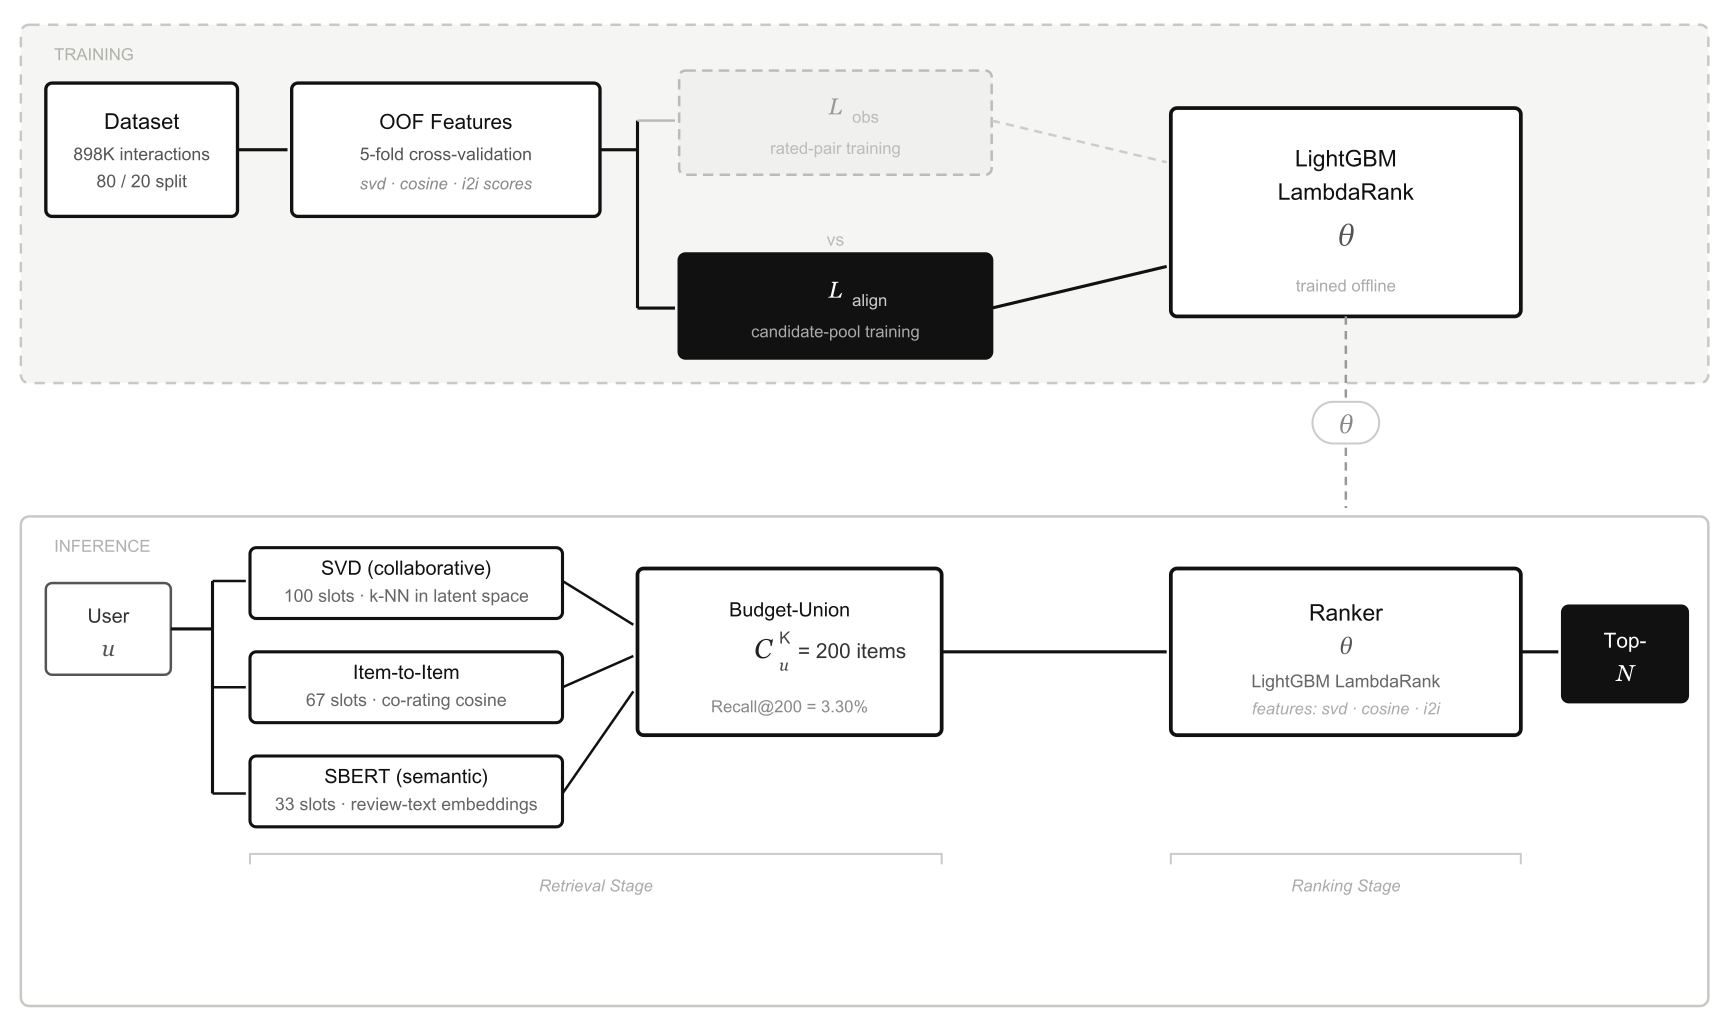
\includegraphics[width=\linewidth]{fig_architecture_new.png}
\caption{System architecture. SVD, SBERT and item-to-item signals feed a
budget-union candidate pool of 200 items. A LightGBM LambdaRank ranker trained
on out-of-fold features produces the final list.}
\label{fig:arch}
\end{figure}

Figure~\ref{fig:arch} shows the system architecture. Data flows from the raw
Amazon dataset through a $k$-core filter and a per-user split into two parallel
stages.

\subsection{Dataset and Preprocessing}
\label{sec:data}

We use the Amazon Electronics Reviews 2023 dataset \citep{hou2024bridging}. A
raw sample of 2{,}000{,}000 reviews is drawn and filtered with a 5-core
procedure, retaining only users and items with at least five interactions,
applied iteratively to convergence. The resulting dataset contains 898{,}387
interactions, 79{,}838 users and 48{,}154 items at a density of 0.0234\%.
Ratings are heavily skewed toward five stars. Identifiers are encoded as
contiguous integers, and review text is lowercased and stripped of
punctuation. The $k$-core filter removes the cold-start population by
construction, so cold-start evaluation is conducted separately on the
unfiltered data (Section~\ref{sec:cold}). Table~\ref{tab:data} summarises the
dataset.

\begin{table}[!ht]
\centering
\caption{Dataset statistics after iterative 5-core filtering. The split is
performed per user, so it does not land on exactly 80/20.}
\label{tab:data}
\small
\begin{tabularx}{\linewidth}{Lr}
\toprule
Statistic & Value \\
\midrule
Raw reviews sampled        & 2{,}000{,}000 \\
After 5-core filter        & 898{,}387 \\
Unique users               & 79{,}838 \\
Unique items               & 48{,}154 \\
Interaction density        & 0.0234\% \\
Training interactions      & 721{,}704 (80.3\%) \\
Test interactions          & 176{,}683 (19.7\%) \\
5-star / 4-star / 3-star   & 67.0\% / 14.7\% / 7.0\% \\
2-star / 1-star            & 4.3\% / 7.1\% \\
\bottomrule
\end{tabularx}
\end{table}

\subsection{Data Split and Leakage Control}
\label{sec:split}

The data is partitioned once, per user, into training and test sets. All
statistics, model parameters and derived features are computed from the
training partition only and applied to the test partition. Features derived
from model predictions are generated out-of-fold using five-fold
cross-validation: for a training row in fold $F_j$, its feature value is
produced by a model trained on all folds except $F_j$. No feature value used
in training is derived from a model that observed the row it describes.

One leakage path specific to the aligned training scheme required attention.
Per-fold retrieval initially excluded each user's training items from the
candidate pool but not their test items, which admitted a small number of test
pairs into the training candidates as negatives. These were false negatives
that biased the ranker against test items rather than toward them. All such
pairs were removed, and the fold candidates were verified to contain no test
pair before training. We describe the protocol as leakage-controlled rather
than leakage-free, because the guarantee rests on checks we performed rather
than on an argument that no path can exist.

\subsection{Feature Signals}
\label{sec:features}

\textbf{Collaborative signal.} Singular value decomposition is applied to the
user-item rating matrix \citep{koren2009matrix}. User $u$ and item $i$ are
represented by latent vectors $p_u$ and $q_i$ in a shared space of dimension
$d=50$:
\begin{equation}
\hat{y}_{ui} = p_u^{\top} q_i .
\end{equation}
The inner product serves as both a retrieval signal and a ranking feature.

\textbf{Semantic signal.} Each item is represented by a 384-dimensional
embedding of its review text, encoded with Sentence-BERT
\citep{reimers2019sentence}. A user is represented by the mean embedding of
their highly-rated training items. Cosine similarity provides the semantic
ranking feature and a retrieval source.

\textbf{Item-to-item signal.} For each item, nearest neighbours are identified
from co-rating patterns in the training partition using cosine similarity over
item columns of the rating matrix \citep{sarwar2001item}. The neighbour table
serves as a retrieval source and the similarity score as a ranking feature.

\subsection{Stage 1: Retrieval}
\label{sec:retrieval}

The retrieval stage produces, for each user, a candidate set of 200 items.
Candidates are drawn from each signal under a fixed budget: 100 slots for the
collaborative source, 67 for the item-to-item source and 33 for the semantic
source. The candidate set is the union of the top items from each source up to
its budget. Unused slots are redistributed, and remaining slots are filled
with popular items from the training partition. Retrieval quality is measured
by Recall@$K$:
\begin{equation}
\mathrm{Recall}@K = \frac{1}{|U|}\sum_{u \in U}
\frac{\left|\mathcal{C}^{K}_{u} \cap \mathcal{R}_{u}\right|}
     {\left|\mathcal{R}_{u}\right|} .
\end{equation}

\subsection{Stage 2: Ranking}
\label{sec:ranking}

The ranking model is a LightGBM ranker \citep{ke2017lightgbm} trained in
LambdaRank mode \citep{burges2010ranknet}, optimising a ranking objective
derived from NDCG. Training data is grouped by user. Features for each
user-item pair are the collaborative score, semantic score, item-to-item
score, item popularity and user activity. Raw identifiers are not used as
features.

We compare two training schemes. Under \emph{observed-pair} training, the loss
is computed over items users actually rated:
\begin{equation}
\Lobs = \sum_{u \in U} \sum_{(u,i,j) \in \mathcal{O}_u} \lambda(u,i,j) .
\end{equation}
Under \emph{aligned} training, the loss is computed over the candidates
retrieval produces:
\begin{equation}
\Lalign = \sum_{u \in U} \sum_{(u,i,j) \in \mathcal{C}_u} \lambda(u,i,j) .
\end{equation}
The two schemes use the same model, features and loss function, and differ
only in the set of items the loss is computed over. To generate aligned
training candidates without leakage, retrieval for training data is performed
out-of-fold following Section~\ref{sec:split}.

Labels within each user's retrieved training pool are binary. A candidate the
user rated 5 in the fold's held-out rows is labelled relevant, and every other
candidate is labelled non-relevant, including items the user rated lower and
items the user never rated. Users with no relevant candidate in their pool are
dropped from training, since LambdaRank has no pairwise signal for them.

\begin{figure}[!ht]
\centering
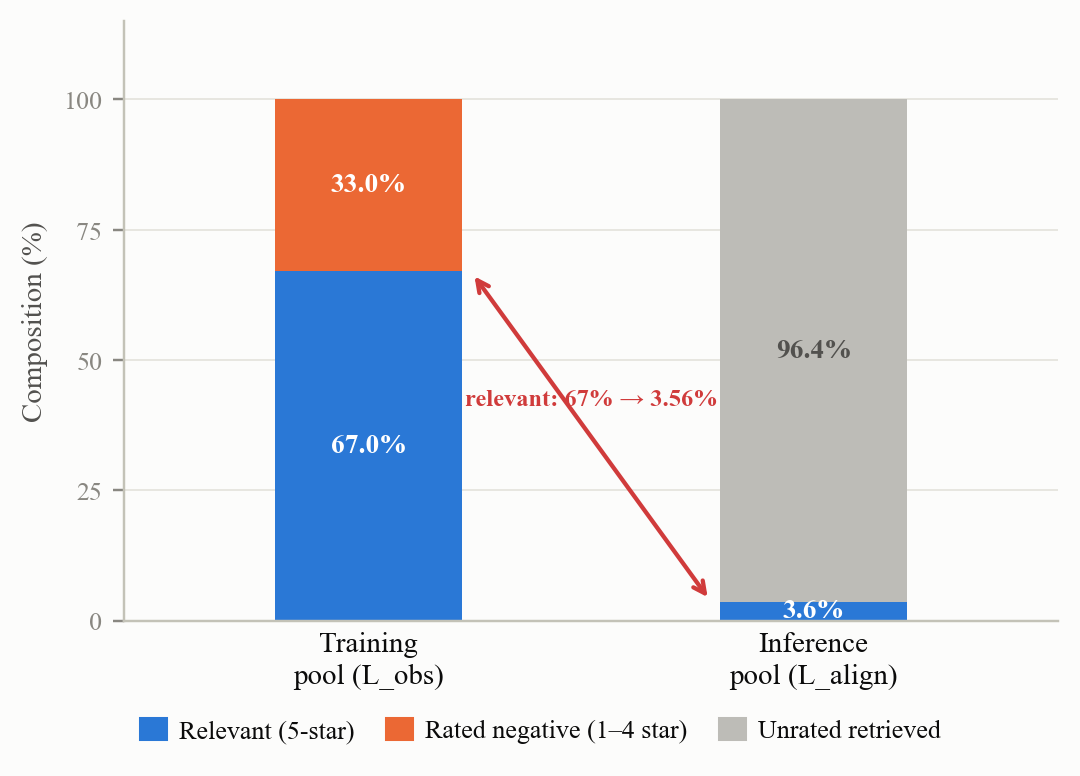
\includegraphics[width=\linewidth]{fig_mismatch_schematic.png}
\caption{Training pool ($\Lobs$) versus inference pool. At training, 67\% of
items are 5-star rated. At inference, only 3.30\% of held-out positives reach
the candidate pool. When one is retrieved, the surrounding candidates are
predominantly items the user never rated, and so differ substantially from the
observed pairs used under observed-pair training.}
\label{fig:mismatch}
\end{figure}

Figure~\ref{fig:mismatch} illustrates the mismatch. At training time every
item in a user's history was chosen by that user, so the task the model
practises is to separate liked items from other rated items. At inference the
pool is dominated by unrated retrieved candidates, and the task differs in
kind.

\subsection{Evaluation Protocol}
\label{sec:eval}

Ranking metrics are computed against candidate lists of one relevant item and
99 sampled items the user did not rate. An item is relevant when its rating
equals 5. The primary metric is NDCG@$K$ \citep{jarvelin2002cumulated}:
\begin{align}
\mathrm{NDCG}@K &= \frac{\mathrm{DCG}@K}{\mathrm{IDCG}@K}, \nonumber\\[2pt]
\mathrm{DCG}@K  &= \sum_{j=1}^{K}\frac{\mathrm{rel}_j}{\log_2(j+1)} .
\end{align}

We also report HR@$K$ and MRR. Following \citet{krichene2020sampled}, sampled
metrics are interpreted as approximations, and Section~\ref{sec:variance}
quantifies their sensitivity to the draw of negatives.

Several signals are heavily tied, since item popularity is an integer count
and the item-to-item score is zero for any item without co-rating neighbours.
Tie handling matters: breaking ties optimistically moves the item-to-item
baseline from 0.1576 to 0.2170 at HR@10. We therefore take the exact
expectation under uniformly random tie-breaking. With $g$ candidates scoring
strictly higher and $e$ scoring equal, the positive occupies rank $g+1+j$ for
$j = 0,\dots,e$ with equal probability, giving
\begin{equation}
\mathrm{HR}@k = \frac{\left|\{\,j : g+1+j \le k\,\}\right|}{e+1} ,
\end{equation}
with NDCG and MRR averaged the same way.

Two denominators appear in this paper and are labelled wherever used.
\emph{Retrieved-only} conditions on retrieval success, so it describes the
ranker given a pool that contains the held-out item, and covers 3{,}914
positives. \emph{All users} charges retrieval misses to the system by scoring
a missed positive outside the pool, and covers 118{,}464 positives. The two
answer different questions and are never mixed within a table.

The system is evaluated at three levels: end-to-end, with negatives drawn from
the retrieval pool; in isolation, with the ranker evaluated against
full-catalogue negatives independently of retrieval; and retrieval recall. For
cold-start, the evaluation uses the same protocol on a separate dataset
constructed from the unfiltered source, with a relevance threshold of
rating $\ge 4$ for cold items.

\subsection{Baselines}
\label{sec:baselines}

Six baselines are evaluated. Popularity isolates the non-personalised floor,
SVD the collaborative signal alone, item-to-item the co-occurrence signal
alone, and SBERT the pretrained semantic signal. TF-IDF and a convolutional
encoder trained on this data isolate term-frequency and non-pretrained
learned text representations respectively. SBERT exceeded both
(HR@10 0.1565 against 0.1131 and 0.1160 on the earlier priority-fill pool),
which is the expected ordering when the training corpus is small relative to
what a pretrained encoder has already seen. Because those two were not
rescored on the final pool, they are excluded from
Table~\ref{tab:main} and that comparison is reported here only.

All remaining baselines are scored on the same budget-union candidate pool as
the hybrid system, so every method faces the same recall ceiling and the same
evaluation set. We considered EASE \citep{steck2019embarrassingly} but its
$|I| \times |I|$ Gram inverse needs roughly 18.6\,GB at $|I| = 48{,}154$, and
restricting the catalogue to fit would have left only 57.7\% of pool rows
scorable, handicapping it rather than testing it. As reported below, the
popularity baseline turns out to be the strongest of those tested, which is
the pattern \citet{dacrema2019really} describe.

% =============================================================================
\section{Results}
\label{sec:results}

\subsection{Retrieval is the Dominant Bottleneck}
\label{sec:bottleneck}

The claims in this section are scoped to this catalogue, this candidate budget
and this evaluation protocol. Within that configuration, retrieval emerges as
the dominant observed bottleneck.

Table~\ref{tab:main} reports end-to-end results for all methods on the
budget-union pool. Each value is the mean over five draws of the negative
sample, with the standard deviation across draws in parentheses.

\begin{table*}[t]
\centering
\caption{End-to-end results on the budget-union pool, conditioned on retrieval
success (3{,}914 positives). Each value is the mean over five draws of the
negative sample, with the standard deviation across draws in parentheses.
Ties are resolved by exact expectation under random tie-breaking.}
\label{tab:main}
\small
\begin{tabularx}{\textwidth}{Lccccc}
\toprule
Model & HR@1 & HR@5 & HR@10 & NDCG@10 & MRR \\
\midrule
Popularity             & 0.1346 (0.0030) & 0.3574 (0.0035) & 0.5078 (0.0022) & 0.2969 (0.0016) & 0.2544 (0.0020) \\
SVD (collaborative)    & 0.0423 (0.0021) & 0.1377 (0.0007) & 0.1996 (0.0021) & 0.1106 (0.0017) & 0.1027 (0.0015) \\
Item-to-item           & 0.0300 (0.0009) & 0.0945 (0.0022) & 0.1576 (0.0014) & 0.0823 (0.0007) & 0.0821 (0.0004) \\
SBERT (semantic)       & 0.0145 (0.0009) & 0.0591 (0.0009) & 0.1086 (0.0030) & 0.0524 (0.0010) & 0.0595 (0.0004) \\
Hybrid (observed-pair) & 0.0434 (0.0017) & 0.1093 (0.0015) & 0.1704 (0.0018) & 0.0964 (0.0010) & 0.0947 (0.0013) \\
\midrule
Hybrid (aligned)       & \textbf{0.1508} (0.0040) & \textbf{0.4166} (0.0033) & \textbf{0.5687} (0.0018) & \textbf{0.3366} (0.0017) & \textbf{0.2844} (0.0022) \\
\bottomrule
\end{tabularx}
\end{table*}

The comparison against the popularity baseline turns on how the ranker is
trained, and we state both directions plainly. Popularity beats the
observed-pair ranker decisively, 0.5078 against 0.1704, a factor of three.
Popularity loses to the aligned ranker, 0.5078 against 0.5687, a difference of
$+0.0610$ with a standard deviation of 0.0029 across negative-sample draws and
a range of $+0.0574$ to $+0.0648$, positive under every draw tested. A
non-personalised baseline therefore outperforms this system when the ranker is
trained on observed pairs, and does not outperform it once the ranker is
trained on the distribution it must serve. Popularity is also the strongest
baseline of the six, ahead of every personalised single signal, which
reproduces on this data the pattern \citet{dacrema2019really} report.

Popularity's strength is not structural access to the catalogue, since it is
scored on the same retrieved pool as every other method. Two effects appear to
explain it. First, the sampled-negative protocol favours popularity by
construction: a held-out five-star item sits at the 83rd percentile of its own
candidate pool's popularity distribution on average, and in the top decile in
50.8\% of cases, with a median training popularity of 225 interactions against
a pool mean of 87. Ranking by popularity therefore exploits a regularity the
protocol introduces rather than a preference it discovers, which is the
concern \citet{krichene2020sampled} raise about sampled metrics. Second, the
observed-pair ranker is not a fair representative of the ranking stage, for
the reason Section~\ref{sec:align} establishes.

The ranking model in isolation achieves HR@10 of 0.1701 against full-catalogue
negatives across 62{,}787 users. This is the harder task, because the ranker
competes against all 48{,}154 items rather than a 200-item pool and every test
user is evaluated rather than only those whose held-out item was retrieved.

Retrieval recall is the binding quantity. Under the initial combination
strategy, which filled the candidate set from the collaborative source first,
recall at 200 candidates was 2.61\%, and the item-to-item and semantic sources
contributed zero candidates on average across all users.
Table~\ref{tab:recall} reports recall and slot allocation under both
strategies. Switching to a fixed budget-union allocation raises recall from
2.61\% to 3.30\%, a 26\% relative increase, because the sources were
complementary and the earlier combination wasted them. All results in this
paper use budget-union retrieval.

\begin{table}[!ht]
\centering
\caption{Retrieval recall and average slot allocation under priority-fill
versus budget-union. Priority-fill excludes the item-to-item and semantic
sources entirely. Slot counts are per-user averages out of 200.}
\label{tab:recall}
\small
\begin{tabularx}{\linewidth}{Lcccc}
\toprule
Strategy & Recall & SVD & I2I & SBERT \\
\midrule
Priority-fill & 2.61\% & 199.5 & 0.0  & 0.0  \\
Budget-union  & 3.30\% & 100.0 & 66.7 & 32.9 \\
\bottomrule
\end{tabularx}
\end{table}

Even after correction, recall remains low. Figure~\ref{fig:recall} shows that
recall grows sublinearly with candidate-set size $K$. The signals impose
ceilings on sparse data that combination alone does not lift.

\begin{figure}[!ht]
\centering
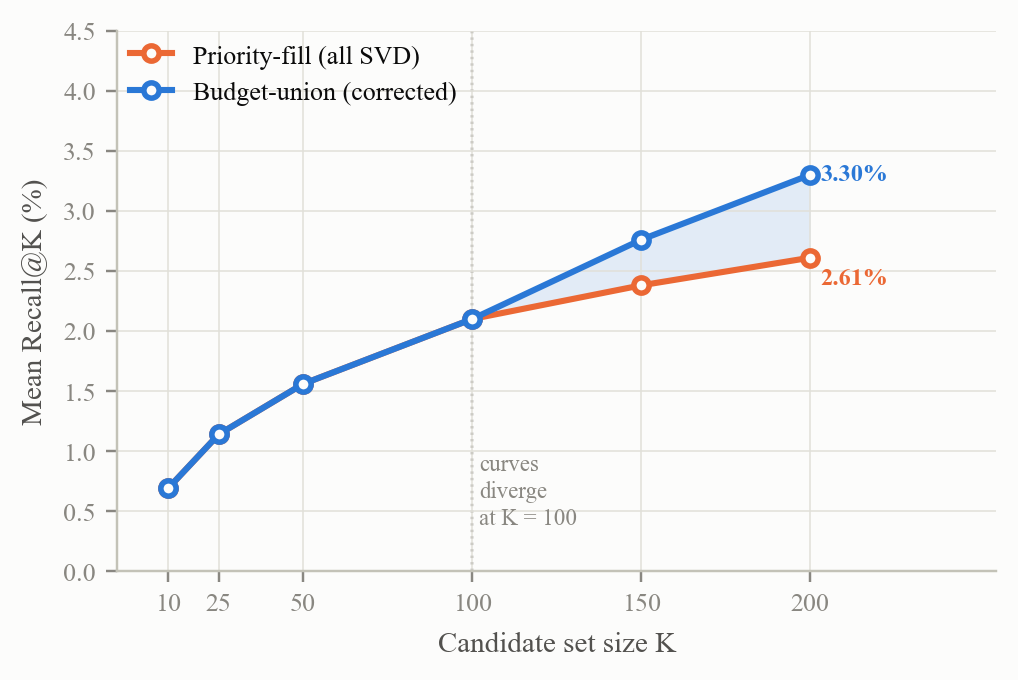
\includegraphics[width=\linewidth]{fig_recall_curve.png}
\caption{Recall@$K$ under priority-fill (orange, dashed) versus budget-union
(blue, solid). Budget-union raises Recall@200 from 2.61\% to 3.30\% by
guaranteeing slots to all three sources. Both curves grow sublinearly.}
\label{fig:recall}
\end{figure}

\subsection{Training-Serving Alignment}
\label{sec:align}

Table~\ref{tab:align} reports the ranking model under both training schemes
evaluated in isolation, so the comparison reflects ranking quality rather than
the quality of the retrieval pool.

\begin{table}[!ht]
\centering
\caption{Hybrid ranker under observed-pair versus aligned training, evaluated
in isolation (62{,}787 users, full-catalogue negatives).}
\label{tab:align}
\small
\begin{tabularx}{\linewidth}{Lccccc}
\toprule
Scheme & HR@1 & HR@5 & HR@10 & NDCG@10 & MRR \\
\midrule
Observed-pair & 0.0376 & 0.1135 & 0.1701 & 0.0939 & 0.0872 \\
Aligned       & 0.1926 & 0.4047 & 0.5167 & 0.3392 & 0.3015 \\
$\Delta$      & $+0.155$ & $+0.291$ & $+0.347$ & $+0.245$ & $+0.214$ \\
\bottomrule
\end{tabularx}
\end{table}

Trained on observed rated pairs, the ranker places a relevant item in a user's
top ten for 17\% of users. Trained on retrieved candidates, the same model
does so for 52\% of users. NDCG@10 rises from 0.0939 to 0.3392 and MRR from
0.0872 to 0.3015. The model, features and evaluation are identical, and only
the set of items the ranker learns to order differs.

The mechanism is direct. Under observed-pair training the ranker learns to
separate relevant rated items from other rated items, a comparison it never
faces at inference. At inference it must separate a relevant item from
retrieved candidates, most of which the user never rated, and it has no
training signal for that comparison. Aligned training replaces the wrong
question with the right one, and the improvement requires no more powerful
model.

The gain is bounded end-to-end by retrieval. With 3.30\% recall most relevant
items remain absent from the candidate pool regardless of how well the ranker
orders what it receives. Training-serving alignment is the most effective
single improvement we found available to the ranking stage, but it is not a
substitute for improving retrieval.

\subsubsection*{What the aligned ranker learns}

The mechanism above says the ranker is asked a different question under each
scheme. Feature attributions show what it answers with.
Figure~\ref{fig:featimp} reports each feature's share of total split gain.

\begin{figure*}[t]
\centering
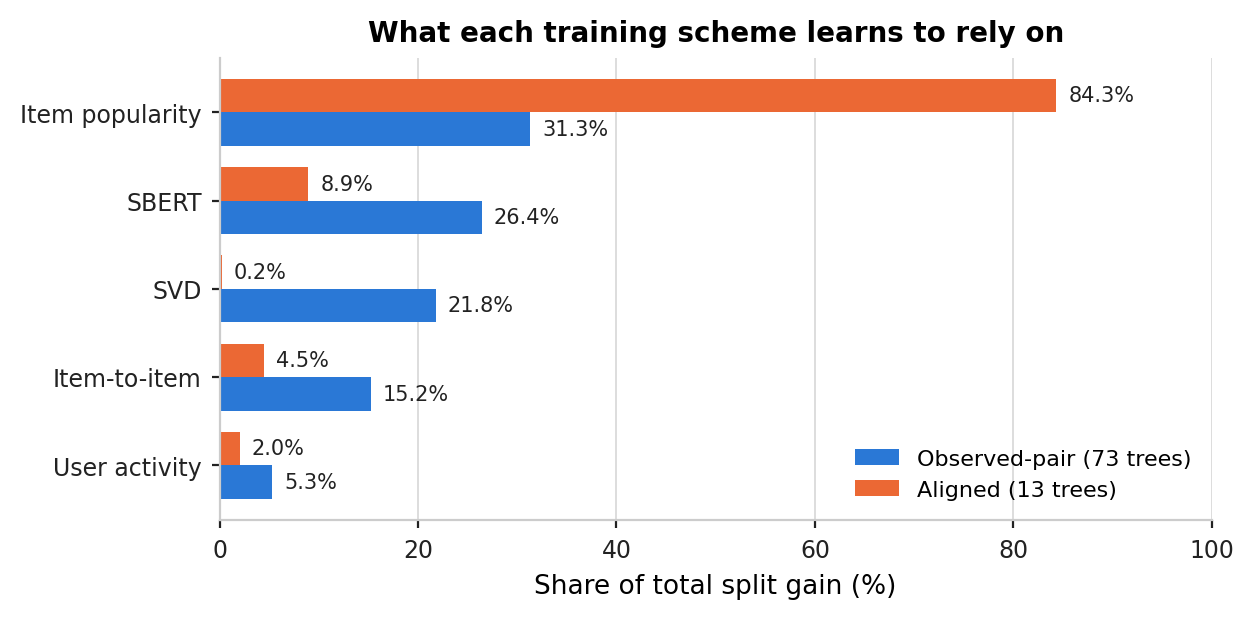
\includegraphics[width=0.78\textwidth]{fig_feature_importance.png}
\caption{Share of total LightGBM split gain per feature under each training
scheme. Aligned training concentrates 84.3\% of gain on item popularity and
reduces the collaborative signal to 0.2\%, and it reaches its stopping point
in 13 trees rather than 73.}
\label{fig:featimp}
\end{figure*}

The shift is large and one-directional. Item popularity rises from 31.3\% of
gain under observed-pair training to 84.3\% under aligned training, while the
collaborative signal falls from 21.8\% to 0.2\%, the semantic signal from
26.4\% to 8.9\% and the item-to-item signal from 15.2\% to 4.5\%. The aligned
model also reaches its stopping point after 13 boosting rounds against 73, so
the function it settles on appears to be both popularity-dominated and simple.

This qualifies the accuracy result and should be read alongside it. On this
evidence, aligned training does not teach the ranker a richer use of the
collaborative and semantic signals. It appears to teach the ranker a
popularity prior and a correction to it, because in a pool of mostly unrated
retrieved candidates popularity is the feature that best separates the rare
relevant item from the rest. The margin over the popularity baseline in
Table~\ref{tab:main}, $+0.0610$ at HR@10, is the value added by the remaining
15.7\% of gain once that prior is learned. The margin is robust, as
Section~\ref{sec:variance} establishes, but it is a smaller claim than the
factor of three over observed-pair training suggests on its own, and we state
both.

The attribution also explains the diversity cost directly rather than by
inference. Learning from retrieved candidates teaches the ranker that popular
items are most likely to be relevant, since they appear most often in
retrieval, which is the popularity bias documented by
\citet{abdollahpouri2021user}. Table~\ref{tab:diversity} reports
beyond-accuracy metrics. Among models with competitive accuracy the pretrained
SBERT encoder achieves the lowest concentration (Gini 0.8623) and high novelty
(14.49), contrasting with the aligned hybrid (Gini 0.9968). A model drawing
84\% of its discriminative power from popularity would be expected to
concentrate its recommendations on popular items, and it does.

\begin{table}[!ht]
\centering
\caption{Beyond-accuracy metrics at $K=10$. ILD is intra-list diversity
(higher is more diverse). Novelty is mean $-\log_2(\text{pop.})$ (higher is
more novel). Gini is concentration (higher is more concentrated). Computed on
the ranked lists from the priority-fill evaluation, so values are comparable
between models but not to Table~\ref{tab:main}.}
\label{tab:diversity}
\small
\begin{tabularx}{\linewidth}{Lccc}
\toprule
Model & ILD & Novelty & Gini \\
\midrule
Popularity             & 0.8624 & 9.89  & 0.9989 \\
SVD (collaborative)    & 0.8701 & 12.21 & 0.9552 \\
Item-to-item           & 0.8694 & 12.09 & 0.9465 \\
SBERT (semantic)       & 0.6672 & 14.49 & 0.8623 \\
TF-IDF                 & 0.8682 & 11.78 & 0.9534 \\
CNN (trained on data)  & 0.8600 & 14.60 & 0.8367 \\
Hybrid (observed-pair) & 0.8853 & 13.76 & 0.9245 \\
Hybrid (aligned)       & 0.8399 & 10.32 & 0.9968 \\
\bottomrule
\end{tabularx}
\end{table}

\subsection{Cold-Start Scale and Asymmetry}
\label{sec:cold}

A cold user or cold item is one with between one and four interactions in the
raw data, and therefore absent from the 5-core clean set. The warm-core
evaluation above characterises the minority of the data.
Table~\ref{tab:cold} reports the scale of the cold and warm populations and
cold-start retrieval results. Cold users account for 69.7\% of all users and
cold items for 82.9\% of all items, so the cold regime is the dominant
operating condition of a deployed system. Figure~\ref{fig:cold} shows the
asymmetry across interaction-count bins.

\begin{table}[!ht]
\centering
\caption{Cold-start evaluation. Cold-item results cover 187{,}862 testable
items through 3{,}919 warm-user test pairs, with a relevance threshold of
$\ge 4$. A dash marks a metric that is undefined because the signal returns
no candidates at all.}
\label{tab:cold}
\small
\begin{tabularx}{\linewidth}{Lccc}
\toprule
Method & HR@10 & NDCG@10 & MRR \\
\midrule
\multicolumn{4}{@{}l}{\textit{Cold items} (82.9\% of the catalogue)} \\
\quad SBERT (semantic) & 0.1967 & 0.0957 & 0.0891 \\
\quad SVD              & 0      & ---    & ---    \\
\quad Item-to-item     & 0      & ---    & ---    \\
\midrule
\multicolumn{4}{@{}l}{\textit{Cold users} (69.7\% of all users)} \\
\quad SBERT profile    & 0.1563 & 0.0804 & 0.0807 \\
\quad Popularity       & 0.5869 & 0.3995 & 0.3571 \\
\bottomrule
\end{tabularx}
\end{table}

For cold items the semantic signal achieves HR@10 of 0.1967, above the random
baseline of 0.10. The collaborative and item-to-item signals score zero by
construction, because an item with no interaction history has no latent
factors and no co-rating neighbours. The semantic signal is the only retrieval
channel available for cold items, and it appears effective precisely because
it operates on review text rather than interaction history.

For cold users a preference profile built from very few interactions achieves
HR@10 of 0.1563, well below the popularity baseline at 0.5869. With a handful
of interactions the averaged preference representation is unstable and does
not converge on a reliable direction. The popularity baseline, which ignores
the user entirely, is more reliable at this level of sparsity.

The asymmetry appears structural. An item's review text exists regardless of
its interaction history, so a useful representation is available from the
moment the item enters the catalogue. A cold user's few interactions do not
describe a stable preference, so no comparable representation can be formed
from them alone. Cold items and cold users present different problems
requiring different remedies.

\begin{figure*}[t]
\centering
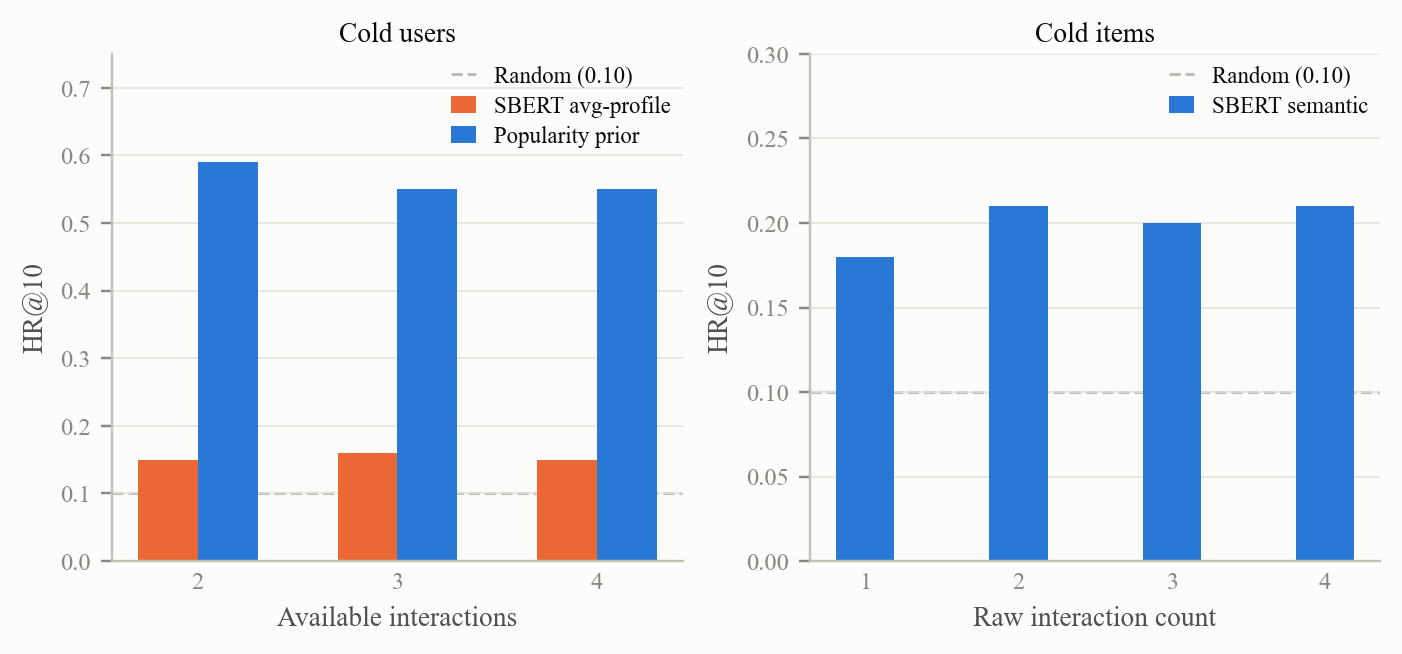
\includegraphics[width=0.92\textwidth]{fig26_coldstart_warmup.png}
\caption{Cold-start results by available interaction count. Left, popularity
dominates cold-user recommendation at every sparsity level. Right, SBERT
retrieves cold items above the random baseline even with a single
interaction.}
\label{fig:cold}
\end{figure*}

% =============================================================================
\section{Diagnostic Experiments}
\label{sec:diagnostics}

The results above establish that the aligned ranker outperforms the
observed-pair ranker and that retrieval recall is low. They do not establish
how much of the remaining error each stage owns. This section reports three
experiments that separate the two contributions. All three use the all-users
denominator, so a retrieval miss counts against the system.

\subsection{Oracle and Near-Oracle Retrieval}
\label{sec:oracle}

Retrieval and ranking failures are confounded in end-to-end metrics. A user
whose held-out item never enters the candidate pool is scored as a miss, and
that miss is attributed to the system as a whole. To separate the two we
inject the held-out positive into the pool for a controlled fraction of users
and leave the ranker unchanged.

For injection probability $p$, each test user whose positive is absent from
the pool receives it with probability $p$. Injection displaces the
lowest-scored candidate, so pool size stays fixed at 200. The injected item is
scored by the same trained aligned ranker, using features computed from
training-partition statistics only, so the ranker still decides the item's
rank. No retraining occurs. Setting $p=0$ reproduces the end-to-end result and
$p=1$ is the oracle condition where every positive is retrievable.

\begin{figure*}[t]
\centering
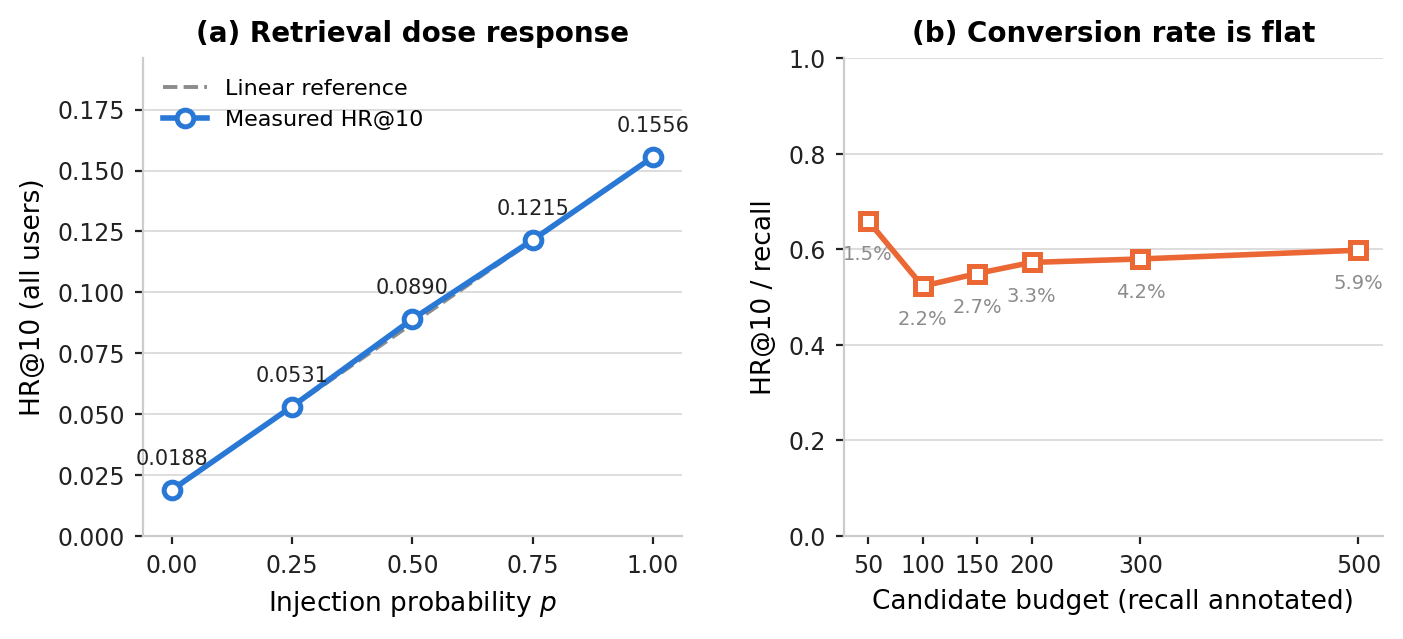
\includegraphics[width=0.92\textwidth]{fig_oracle_injection.png}
\caption{(a) HR@10 against injection probability, against a straight reference
line drawn between the endpoints. The measured response is close to linear, so
recall converts to ranking gain at a near-constant rate. (b) The conversion
rate, aligned HR@10 divided by recall, with recall annotated at each budget. A
tenfold increase in pool size does not reduce the rate at which a retrieved
positive becomes a top-ten hit.}
\label{fig:oracle}
\end{figure*}

Oracle retrieval raises HR@10 from 0.0188 to 0.1556, a factor of 8.3, without
touching the ranker, and MRR from 0.0142 to 0.0824. Retrieval therefore owns
the large majority of end-to-end error on this catalogue, which is consistent
with the diagnosis from recall alone.

The shape of the response matters as much as its size. HR@10 increases by
0.0343, 0.0359, 0.0325 and 0.0341 across the four successive steps in $p$, and
Figure~\ref{fig:oracle}(a) plots this against a straight line between the
endpoints. The response is close to linear, so each marginal unit of recall
converts to ranking gain at a near-constant rate, and we observe no region of
diminishing returns within the measured range. Investment in retrieval would
not saturate at this operating point.

The oracle condition also bounds the ranker. With the positive guaranteed
present in a pool of 200, the ranker places it in the top ten for only 15.56\%
of users, leaving the correct item outside the top ten in roughly 84\% of
cases where that item is available to be found. Retrieval dominates, but the
ranker is independently weak, and fixing retrieval alone would not produce a
strong system. We report both facts because the second qualifies the first.

\subsection{Variance: Initialisation and Negative Sampling}
\label{sec:variance}

Single-run differences can reflect initialisation or the draw of negatives
rather than method, so we quantify both across the seeds
$\{42, 123, 456, 789, 1000\}$.

Retraining the aligned ranker five times on identical out-of-fold data gives
HR@10 of 0.0188 with a standard deviation of 0.00009. Alignment moves HR@10
from 0.0056 to 0.0188 over that denominator, a gap of 0.0132 that exceeds
initialisation noise by more than two orders of magnitude.

Initialisation is not the dominant source of noise, however. Every metric here
comes from scoring one positive against 99 sampled negatives, and sampled
metrics are known to be unreliable \citep{krichene2020sampled}. Repeating the
evaluation with five sampling seeds, holding every model fixed and giving all
methods the same draw within each seed, moves HR@10 by about 0.002: roughly
twenty times the initialisation figure. Reporting initialisation variance
alone would therefore understate uncertainty by an order of magnitude. Both
effects survive comfortably. The aligned advantage over popularity is 0.0610
with a standard deviation of 0.0029, so some twenty-one times that noise, and
it is positive under every seed tested; the advantage over the observed-pair
ranker is larger still. Neither comparison depends on a fortunate draw.

\subsection{Candidate Budget Ablation}
\label{sec:budget}

Figure~\ref{fig:recall} reports recall as a function of budget but does not
show whether added candidates translate into ranking gains or merely add
noise. We therefore reran the full pipeline end to end at six budgets and
scored each pool with both rankers.

\begin{table}[!ht]
\centering
\caption{End-to-end budget ablation, all users denominator. Recall is the
fraction of held-out positives entering the pool. Conv.\ is aligned HR@10
divided by recall, the rate at which retrieved positives become top-ten hits.
The budget-200 row comes from a separate run from
Section~\ref{sec:oracle} and agrees with it to within the sampling noise
quantified in Section~\ref{sec:variance}.}
\label{tab:budget}
\small
\begin{tabularx}{\linewidth}{Lccccc}
\toprule
& & \multicolumn{2}{c}{Observed-pair} & \multicolumn{2}{c}{Aligned} \\
\cmidrule(lr){3-4}\cmidrule(lr){5-6}
Budget & Recall & HR@10 & NDCG@10 & HR@10 & Conv. \\
\midrule
50  & 1.47\% & 0.0042 & 0.0024 & 0.0097 & 0.66 \\
100 & 2.18\% & 0.0042 & 0.0024 & 0.0114 & 0.52 \\
150 & 2.73\% & 0.0053 & 0.0031 & 0.0150 & 0.55 \\
200 & 3.30\% & 0.0056 & 0.0032 & 0.0189 & 0.57 \\
300 & 4.19\% & 0.0070 & 0.0039 & 0.0243 & 0.58 \\
500 & 5.85\% & 0.0088 & 0.0047 & 0.0350 & 0.60 \\
\bottomrule
\end{tabularx}
\end{table}

Three patterns emerge. First, retrieval scales sublinearly. A tenfold budget
increase from 50 to 500 raises recall by a factor of four, from 1.47\% to
5.85\%, so widening the pool is a weakening lever.

Second, and against the usual expectation, added candidates do not appear to
dilute ranking quality. The conversion rate is 0.66, 0.52, 0.55, 0.57, 0.58
and 0.60 across the six budgets, plotted in Figure~\ref{fig:oracle}(b). It is
flat and drifts slightly upward rather than falling. A pool ten times larger
contains ten times the distractors, yet the ranker's conversion rate does not
degrade. Read together with Section~\ref{sec:oracle}, this locates the ceiling
in recall rather than in ranker capacity under load. It is also consistent
with what Figure~\ref{fig:featimp} shows the ranker relies on, since a
popularity prior does not become less discriminative as the pool grows.

Third, the benefit of alignment grows with budget. The aligned HR@10 advantage
over the observed-pair ranker is 2.3$\times$ at budget 50, 3.4$\times$ at
budget 200 and 4.0$\times$ at budget 500. This follows from the mismatch
mechanism: a larger pool holds proportionally more unrated candidates, exactly
the items the observed-pair ranker never trained to discriminate, so its
disadvantage compounds as the pool grows.

We omit MRR from Table~\ref{tab:budget} deliberately. Our protocol assigns a
non-retrieved positive a rank outside the pool, so a miss contributes $1/51$
at budget 50 but only $1/501$ at budget 500. Because misses dominate at every
budget, MRR is governed by this penalty floor and falls as the budget grows for
reasons unrelated to ranking quality. HR@$K$ and NDCG@$K$ are unaffected,
since a miss at rank 51 and a miss at rank 501 both contribute zero at $K=10$.

% =============================================================================
\section{Discussion}
\label{sec:discussion}

The findings share a common structure. Each identifies a regime in which an
accepted component of two-stage recommenders does not perform as assumed, and
measures the consequence.

The retrieval finding indicates that the architecture's cooperative premise
breaks down when recall is low. The oracle experiment makes this direct: with
the ranker untouched, guaranteeing the held-out item a place in the pool
multiplies HR@10 by 8.3. The 3.30\% ceiling is consistent with the dataset's
0.023\% density, since a random 200-item set contains the held-out item with
probability 0.42\%, so the achieved recall is eight times that floor.

The comparison with a popularity baseline needs care. Popularity is scored on
the same retrieved pool as the hybrid, so it faces the same recall ceiling and
its strength is not structural access to the catalogue. It appears to reflect
two separable things: the sampled-negative protocol rewards popularity because
held-out items are themselves popular, sitting at the 83rd percentile of their
own pool, and the observed-pair ranker is scoring a distribution it never
trained on. Correcting the second reverses the comparison on an unchanged
pool. The general lesson we draw is that a strong non-personalised baseline
can indicate a misconfigured ranker rather than a limit on personalisation,
and distinguishing the two requires holding the candidate pool fixed while
varying only how the ranker was trained.

The alignment finding shows that the gap between training and serving
distributions is a large and concrete quantity. A threefold gain in top-ten
hit rate from a single distributional correction is, on this evidence, worth
attempting before architectural changes are considered.

Two caveats bound how that result should be read. The first is retrieval: with
3.30\% recall, aligning the ranker perfectly does not resolve the bottleneck,
and the oracle experiment shows the converse too, since even with the positive
always present the ranker misses it from the top ten in 84\% of cases.
Alignment and retrieval improvement are complementary and neither alone
suffices. The second is what alignment teaches. The corrected ranker is
popularity-dominated, drawing 84.3\% of its gain from that one feature, so the
description we can support is not that alignment unlocks the collaborative and
semantic signals but that it replaces a ranker asking the wrong question with
one that has learned the right prior. The remaining signals contribute the
margin over popularity rather than the bulk of the gain. A practitioner
adopting this correction should expect a large accuracy improvement
accompanied by a large concentration increase, and should decide whether that
trade is acceptable beforehand.

The cold-start finding reframes the scope of standard evaluations. Systems
optimised on warm-core benchmarks are characterised for the minority of the
data. The cold majority is harder, partly intractable from interaction data
alone, and differently tractable for items than for users. An item's content
exists before any user interacts with it, whereas a user's preference does not
stabilise until enough interactions accumulate. Architectural solutions that
treat the two cases identically do not address the harder one.

\subsection{Scope and Limitations}
\label{sec:limits}

The mechanisms above rest on controlled interventions, where one factor
changes and everything else is held fixed, and we state them generally. The
magnitudes are properties of this system on this catalogue. The factor of 8.3,
the factor of three, the 3.30\% recall and the 0.0610 margin should not be
expected to transfer.

One measurement bears on that. Attributing the bottleneck to sparsity is
testable, so we reran retrieval on a 40{,}000-user subsample of
MovieLens-20M, 5{,}856{,}070 ratings over 14{,}471 items at a density of
1.0117\%, some 43 times that of the Electronics catalogue. Using the same two
interaction-based signals and the same budget of 200, Recall@200 reaches
59.02\% against 3.30\% here, or 43 times the random floor against 8 times. At
that recall the ranker receives the held-out item more often than not and
retrieval stops binding, which is what the claim predicts for a catalogue that
much denser. It is one measurement under a configuration that excludes the
semantic source and moves the relevance threshold, so it speaks to retrieval
recall alone and not to whether the alignment effect transfers.

Four limitations remain. The findings come from a single product category, so
the magnitudes are uncorroborated. The evaluation uses sampled negatives,
which are inconsistent with full-catalogue metrics
\citep{krichene2020sampled}, and Section~\ref{sec:variance} bounds sensitivity
to the draw but not the bias of the protocol itself. The beyond-accuracy
metrics in Table~\ref{tab:diversity} and the TF-IDF and convolutional
encoders were computed on the priority-fill pool, so they are comparable
between models but not to Table~\ref{tab:main}. And no result resamples the
train and test partition, so a single split underlies every figure reported.

% =============================================================================
\section{Conclusion}
\label{sec:conclusion}

This paper evaluated a hybrid two-stage recommender under a
leakage-controlled, stage-separated protocol and produced three findings.

Retrieval recall is the dominant bottleneck on this catalogue. Recall@200 is
only 3.30\%, so the held-out item reaches the candidate pool in a small
minority of evaluation cases. Guaranteeing it a place in the pool raises HR@10
by a factor of 8.3 without altering the ranker, which is direct evidence that
retrieval coverage constrains the system. Recall does not saturate within the
budgets tested, rising to 5.85\% at 500 candidates.

Training-serving alignment is the largest gain we found available. Replacing
rated-pair training with candidate-pool training raises the top-ten hit rate
from 17\% to 52\% in isolation with no change to the model or features, and it
is what decides whether the system outperforms a non-personalised popularity
baseline. On a common pool, popularity beats the observed-pair ranker by a
factor of three and loses to the aligned ranker by 0.0610 at HR@10. Feature
attributions indicate the corrected ranker is popularity-dominated, so the
gain is better described as learning the right prior than as unlocking the
collaborative and semantic signals, and it carries a measurable concentration
cost.

Cold-start is the dominant regime, covering 70\% of users and 83\% of items.
The semantic signal addresses cold items, while cold users require signals
beyond interaction history.

The common implication is that diagnosing which stage limits a system, and in
which regime, is a necessary step before optimising it. The largest gains in
this system came from diagnosis rather than from a more powerful model.

Future work should address the retrieval ceiling through learned dense
retrieval representations \citep{huang2020embedding}, extend the evaluation to
the cold regime as the primary setting, replicate the findings on a second
catalogue with comparable text so the alignment effect can be tested as well
as recall, and explore ranking objectives that balance accuracy against
concentration rather than optimising accuracy alone.

% =============================================================================
\newpage
\bibliography{references}

\end{document}
